\section{Development model}
The workflow for the development is show in figure
\ref{fig:gajski-kuhn-ychart}. In the Gajski-Kuhn Y-model has 3 axis for the
perspectives of the product. It is typical to start from the behavioral axis,
by treating the systems as a black-box, and then to jump back and forth between
the other axis while gravitating towards the origin (project goal).
\begin{figure}[h]
  \centering
  \resizebox{\linewidth}{!}{
    \begin{tikzpicture}[
        font=\ttfamily,
      ]
      \draw[gray] node[
        circle,
        fill = gray,
        minimum size = 2mm,
        outer sep = 0,
        inner sep = 0,
      ] (O) at (0,0) {};

      \foreach \r/\desc in {
        1/{Electrical},
        2/{Logic gates},
        3/{Register transfer},
        4/{Architecture},
        5/{System}
      }{
        \draw[gray, dashed] (O) circle (\r);
        \draw[gray] (90:\r)
          node[
            above = 1mm,
            align = center,
            font = \small\ttfamily,
            fill = white,
          ] {\desc};
      }

      \draw[hsr-mauve, thick] (O) to ++(30:6)
        node[
          above = 3mm,
          align = center,
          text width = 2cm
        ] {\textbf{Structural Perspective}};
      \foreach \r/\desc in {
        1/{Transistors, Wires},
        2/{Gates, Latches, Flip-Flops},
        3/{ALUs, Registers, Memories},
        4/{Subblocks},
        5/{Top blocks, I/O}
      } {
        \draw[hsr-mauve] (30:\r)
          node[
            circle, minimum size = 2mm,
            fill = hsr-mauve,
            outer sep = 0,
            inner sep = 0
          ] {}
          node[
            below right = 2mm,
            align = left,
            font = \small\ttfamily,
            fill = white,
          ] {\desc};
      }

      \draw[hsr-blue, thick] (O) to ++(150:6)
        node[
          above = 3mm,
          align = center,
          text width = 2cm
        ] {\textbf{Behavioral Perspective}};
      \foreach \r/\desc in {
        1/{Transfer functions},
        2/{Truth tables, State graphs},
        3/{Data moves and operations},
        4/{Subtasks},
        5/{Algorithm}
      } {
        \draw[hsr-blue] (150:\r)
          node[
            circle, minimum size = 2mm,
            fill = hsr-blue,
            outer sep = 0,
            inner sep = 0
          ] {}
          node[
            below left = 2mm,
            align = right,
            font = \small\ttfamily,
            fill = white,
          ] {\desc};
      }

      \draw[hsr-lakegreen, thick] (O) to ++(270:6)
        node[
          below = 3mm,
          align = center,
          text width = 2cm
        ] {\textbf{Physical Perspective}};
      \foreach \r/\desc in {
        1/{Mask polygons, Detailed layout},
        2/{Standard cells, Macro cells},
        3/{Placement and routing},
        4/{Floorplan partitioning},
        5/{Chip or board}
      } {
        \draw[hsr-lakegreen] (270:\r)
          node[
            circle, minimum size = 2mm,
            fill = hsr-lakegreen,
            outer sep = 0,
            inner sep = 0
          ] {}
          node[
            right = 2mm,
            align = left,
            font = \small\ttfamily,
            fill = white,
          ] {\desc};
      }

    \end{tikzpicture}
  }
  \caption{
    Gajski-Kuhn Y-chart.
    \label{fig:gajski-kuhn-ychart}
  }
\end{figure}

%% TODO: finish picture
Figure \ref{fig:asic-design-flow} shows a typical flow diagram of how an ASIC device
is designed.
\begin{figure}
  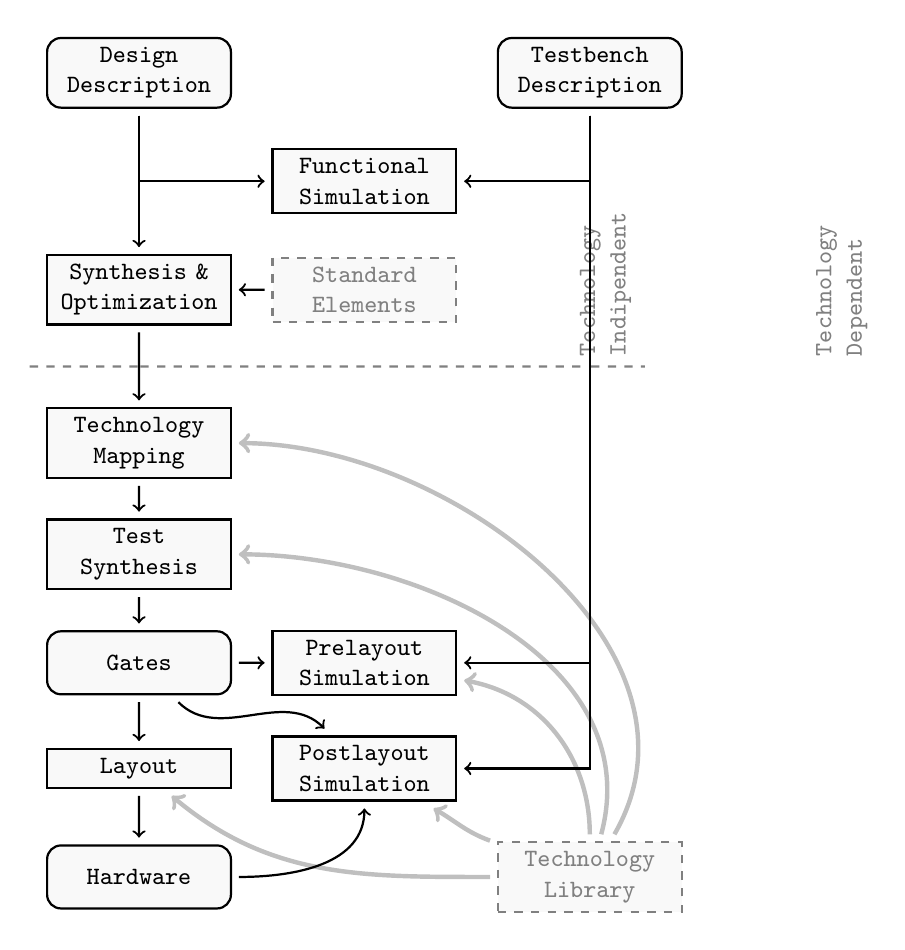
\begin{tikzpicture}[
      scale = .7,
      font = \small\ttfamily,
      bubble/.style = {
        rectangle,
        draw = black, thick,
        fill = lightgray!10,
        align = center,
        text width = 2.1cm,
        rounded corners = 5pt,
        minimum height = 8mm,
        outer sep = 1mm,
      },
      box/.style = {
        rectangle,
        draw = black, thick,
        fill = lightgray!10,
        align = center,
        text width = 2.1cm,
        outer sep = 1mm,
      },
      lib/.style = {
        rectangle,
        draw = black, gray, thick, dashed,
        fill = lightgray!10,
        align = center,
        text width = 2.1cm,
        outer sep = 1mm,
      },
      ghost/.style = {
        outer sep = 0,
        inner sep = 0,
      }
    ]
    \matrix[row sep = 5mm, column sep = 5mm]{
      \node[bubble] (dd) {Design Description}; & & \node[bubble] (tbd) {Testbench Description}; \\
      \node[ghost] (A) {}; & \node[box] (fs) {Functional Simulation}; \\
      \node[box] (so) {Synthesis \& Optimization}; & \node[lib] (se) {Standard Elements}; \\
      \node[ghost] (lineA) {}; & & \node[ghost] (lineB) {}; \\
      \node[box] (tm) {Technology Mapping}; \\
      \node[box] (ts) {Test Synthesis}; \\
      \node[bubble] (gates) {Gates}; & \node[box] (pres) {Prelayout Simulation}; \\
      \node[box] (l) {Layout}; & \node[box] (posts) {Postlayout Simulation}; \\
      \node[bubble] (design) {Hardware}; & & \node[lib] (tech) {Technology Library}; \\
    };

    \draw[thick, dashed, gray]
      (lineA) to ++(-2,0)
      (lineA) to (lineB) to ++(1,0)
      node[rotate = 90, above = 5mm, anchor = west, text width = 3cm]  {\bfseries Technology Indipendent}
      node[rotate = 90, below = 25mm, anchor = west, text width = 3cm] {\bfseries Technology Dependent};

    \begin{scope}[ultra thick, ->, lightgray]
      \draw (tech) to[in = -40, out = 180] (l);
      \draw (tech) to[in = -30, out = 160] (posts);
      \draw (tech) to[in =   0, out =  75] (ts);
      \draw (tech) to[in =   0, out =  60] (tm);
      \draw (tech) to[in = -10, out =  90] (pres);
    \end{scope}

    \begin{scope}[thick, ->]
      \draw (tbd) |- (fs);
      \draw (tbd) |- (pres);
      \draw (tbd) |- (posts);

      \draw (se) -- (so);

      \draw (dd) |- (fs);
      \draw (dd) -- (so);
      \draw (so) -- (tm);
      \draw (tm) -- (ts);
      \draw (ts) -- (gates);

      \draw (gates) -- (pres);
      \draw (gates) to[out = -45, in = 135] (posts);

      \draw (gates) -- (l);
      \draw (l) -- (design);
      \draw (design) to[out = 0, in = -90] (posts);
    \end{scope}

  \end{tikzpicture}
  \caption{
    Design flow for an ASIC device.
    \label{fig:asic-design-flow}
  }
\end{figure}

% \section{Hardware}
%% TODO: hardware

% vim:ts=2 sw=2 et:
